% fA appendix zoom of Figure 2 (b): the two per-band gain controllers at component level.
% (a) SEGA (released) spectral sensor, (b) Constancy-TM. Each is a left-to-right chain from x_t to
% g_{a,j}. Every equation is copied from sec/appendix_impl.tex and Algorithms 1 and 2 (sec/methods.tex);
% the code is crope/sega_official.py and crope/gain.py.
% Build: ~/.local/bin/tectonic -X compile fA_method_zoom.tex -> fA_method_zoom.pdf, 5.50 in wide at
% final print size; include at \linewidth. Coordinates in bp (396 units = 5.50 in), 8 pt grid.
\documentclass[border=0pt]{standalone}
\usepackage{newtxtext}
\usepackage{newtxmath}
\setsansfont{texgyreheros}[Extension=.otf, UprightFont=*-regular, BoldFont=*-bold,
  ItalicFont=*-italic, BoldItalicFont=*-bolditalic]
\renewcommand\familydefault{\sfdefault}
\DeclareMathSizes{7.5}{7.5}{6.1}{6.1}\DeclareMathSizes{9}{9}{6.6}{6.1}
\usepackage{tikz}
\usetikzlibrary{arrows.meta, calc}

% ---------------------------------------------------------------- palette (crope_style.py)
\definecolor{ink}{HTML}{1A1A1A}
\definecolor{ink2}{HTML}{595959}
\definecolor{cMethod}{HTML}{0068A8} \definecolor{cMethodFill}{HTML}{CCE1EE}
\definecolor{cTemp}{HTML}{009870}   \definecolor{cTempFill}{HTML}{CCEAE2}
\definecolor{cLaw}{HTML}{D06008}    \definecolor{cLawFill}{HTML}{F6DFCE}

\newcommand\fsTag{\fontsize{9}{10.8}\selectfont\bfseries}
\newcommand\fsLab{\fontsize{7.5}{8.6}\selectfont}
\newcommand\mean{\operatorname{mean}}
\newcommand\clip{\operatorname{clip}}
\newcommand\std{\operatorname{std}}

\begin{document}
\begin{tikzpicture}[x=1bp, y=1bp, line cap=round, line join=round,
  every node/.style={inner sep=0pt, text=ink, font=\fsLab},
  op/.style={draw=#1, rounded corners=2pt, line width=0.8pt, minimum height=18pt,
    inner xsep=3pt, align=center, anchor=center},
  io/.style={draw=ink, fill=white, rounded corners=2pt, line width=0.8pt, minimum height=18pt,
    inner xsep=3pt, anchor=center},
  flow/.style={-{Stealth[length=3.4pt, width=2.8pt]}, line width=0.6pt, draw=ink},
  wire/.style={line width=0.6pt, draw=ink},
  sym/.style={anchor=south, inner sep=1.2pt},
  tag/.style={font=\fsTag, anchor=base west},
  eq/.style={anchor=base west},
]
\path[use as bounding box] (0,0) rectangle (396,254);

% ================================================================= (a) SEGA spectral sensor
\node[tag] at (0,245) {(a) SEGA spectral sensor};
\def\ya{202}   % main chain
\def\yr{229}   % radial branch
\node[io, minimum width=18pt] (a0) at (9,\ya) {$x_t$};
\node[op=cMethod, fill=cMethodFill, minimum width=46pt] (a1) at (55.9,\ya) {input\\projection};
\node[op=cMethod, fill=cMethodFill, minimum width=34pt] (a2) at (109.7,\ya) {channel\\mean};
\node[op=cMethod, fill=cMethodFill, minimum width=34pt] (a3) at (158.6,\ya) {axis\\profile};
\node[op=cMethod, fill=cMethodFill, minimum width=46pt] (a4) at (213.4,\ya) {pair-to-bin\\map};
\node[op=cMethod, fill=cMethodFill, minimum width=50pt] (a5) at (276.3,\ya) {standardize,\\tanh};
\node[op=cMethod, fill=cMethodFill, minimum width=42pt] (a6) at (337.1,\ya) {allocation};
\node[io, minimum width=22pt] (a7) at (385,\ya) {$g_{a,j}$};
\draw[flow] (a0) -- (a1);
\draw[flow] (a1) -- node[sym] {$h$} (a2);
\draw[flow] (a2) -- node[sym] {$Z$} (a3);
\draw[flow] (a3) -- node[sym] {$E_a$} (a4);
\draw[flow] (a4) -- node[sym] {$\ell_j$} (a5);
\draw[flow] (a5) -- node[sym] {$c_j$} (a6);
\draw[flow] (a6) -- (a7);
% radial branch: spectral flatness of the same map sets the spread
\node[op=cMethod, fill=cMethodFill, minimum width=58pt, minimum height=16pt] (ar) at (213.4,\yr) {radial flatness};
\draw[flow] (a2.north) |- (ar.west);
\draw[flow] (ar.east) -| node[pos=0.75, anchor=west, inner sep=1.5pt] {$\varsigma$} (a6.north);
% equations (sec/appendix_impl.tex, paragraph on the released code; Algorithm 1)
\foreach \x/\y/\e in {
    0/177/{Z=\mean_c h},
    76/177/{K_a=\max(\lfloor L_a/2\rfloor,8)},
    178/177/{\ell_j=\ln E_a\bigl((1-\rho_j)(K_a-1)\bigr)},
    0/164/{\rho_j=j/(D/2-1)},
    76/164/{z_j=(\ell_j-\mean_i\ell_i)/\std_i\ell_i},
    178/164/{c_j=\tanh(1.5z_j)-\mean_i\tanh(1.5z_i)},
    0/151/{\varsigma=1-\mathrm{SF}^{1.5}},
    76/151/{m_{\mathrm{ref}}=\max(s,1)^{0.08}},
    178/151/{m_{a,j}=\max\bigl(1,\,m_{\mathrm{ref}}[1-0.15\,\varsigma\,c_j]\bigr),\ \ g_{a,j}=m_{a,j}^2}}
  \node[eq] at (\x,\y) {$\e$};

% ================================================================= (b) Constancy-TM controller
\node[tag] at (0,130) {(b) Constancy-TM controller};
\def\yg{110}\def\ye{82}\def\ym{96}
\node[io, minimum width=18pt] (b0) at (9,\yg) {$x_t$};
\node[io, minimum width=18pt] (c0) at (9,\ye) {$\hat x_0$};
\node[io, minimum width=42pt, minimum height=16pt] (tg) at (21,54) {$P^{\mathrm{nat}}(f,\sigma)$};
\node[op=cLaw, fill=cLawFill, minimum width=34pt] (b1) at (52,\yg) {band\\energy};
\node[op=cLaw, fill=cLawFill, minimum width=34pt] (c1) at (52,\ye) {band\\energy};
\node[op=cLaw, fill=cLawFill, minimum width=44pt] (b2) at (123,\yg) {visibility\\gate};
\node[op=cLaw, fill=cLawFill, minimum width=44pt] (c2) at (123,\ye) {spectral\\error};
\node[op=cLaw, fill=cLawFill, minimum width=42pt] (b3) at (203,\ym) {correction};
\node[op=cLaw, fill=cLawFill, minimum width=48pt] (b4) at (270,\ym) {interpolate\\in $\log f$};
\node[op=cTemp, fill=cTempFill, minimum width=46pt] (b5) at (339,\ym) {temperature};
\node[io, minimum width=20pt] (b6) at (386,\ym) {$g_{a,j}$};
\draw[flow] (b0) -- (b1);
\draw[flow] (c0) -- (c1);
\draw[flow] (b1) -- node[sym] {$E^x_a[b]$} (b2);
\draw[flow] (c1) -- node[sym] {$\hat E_a[b]$} (c2);
\draw[flow] (tg.east) -| (c2.south);
\draw[wire] (b2.east) -- node[sym] {$w_{a,b}$} (170,\yg) -- (170,\ym+3);
\draw[wire] (c2.east) -- node[sym] {$e_{a,b}$} (170,\ye) -- (170,\ym-3);
\draw[flow] (170,\ym+3) -- (b3.west |- 0,\ym+3);
\draw[flow] (170,\ym-3) -- (b3.west |- 0,\ym-3);
\draw[flow] (b3) -- node[sym] {$\delta_{a,b}$} (b4);
\draw[flow] (b4) -- node[sym] {$\Delta_{a,j}$} (b5);
\draw[flow] (b5) -- (b6);
% equations (sec/appendix_impl.tex, app:laws; Algorithm 2)
\foreach \x/\y/\e in {
    0/30/{\rho_{a,b}=\max\bigl(E^x_a[b]/(\sigma^2C)-1,0\bigr)},
    178/30/{w_{a,b}=\rho_{a,b}/(1+\rho_{a,b})},
    0/17/{e_{a,b}=\tfrac12\bigl(P^{\mathrm{nat}}_a(f_b,\sigma)+c_a-\ln\hat E_a[b]\bigr)},
    178/17/{\delta_{a,b}=\eta\,w_{a,b}\clip(e_{a,b},-1,1)},
    0/4/{\ln g_{a,j}=\ln\tau+\Delta_{a,j}},
    178/4/{\tau=s^{0.16}}}
  \node[eq] at (\x,\y) {$\e$};
\end{tikzpicture}
\end{document}
